\chapter{Query Language}
\label{sec:specification_language}

The centre-piece of the \vnnlib{} standard is the \vnnlib{} query language which is designed as a standardised computer-readable format for expressing a wide range of satisfiability problems over neural networks.
Although the syntax is somewhat human-readable, the syntax of \vnnlib{} is primarily designed with machine-readability in mind. 
It is envisaged that \vnnlib{} queries will primarily be generated automatically by higher level tools that provide human-orientated interfaces.
This chapter describes the syntax, scoping, typing and semantics of the query language.

\section{Syntax}
\label{sec:syntax}

The syntax of the language is shown in Figure~\ref{fig:vnnlib-syntax}.  This section will now describe the key syntactic constructs of the language via illustrative examples. Firstly, \vnnlib{} queries are split into three parts: 
\begin{enumerate}
\item \textbf{Version number} - the version of the VNN-LIB the query is using. This allows tools to provide better diagnostic error messages.
\item \textbf{Network declarations} - a non-empty list of network declarations. This allows the definition of the networks that the satisfiability problem will involve and the definition of new abstract variables that represent the values for the inputs and outputs of the network.
\item \textbf{Assertions} - a list of assertions that reference the variables introduced by the network declarations. This allows the constraints that should be satisfied to be defined.
\end{enumerate}
Currently, the standard does not permit the interleaving of network declarations and assertions. Figure~\ref{fig:simple-query} shows an example of a simple query.

\begin{figure}[p]
	\setlength{\grammarindent}{6.5em}
	
	\begin{grammar}
	<query> ::= <version> [<network>]$^+$ [<assert>]$^*$
	
	<version> ::= (\texttt{vnnlib-version} [0-9]$^+$.[0-9]$^+$)
	
	<name> ::= [A-Za-z][\_A-Za-z0-9]*
		
	<network> ::= (\texttt{declare-network} <name> <equiv>$^?$ <input>$^+$ <hidden>* <output>$^+$)
	
	<equiv> ::= (\texttt{equal-to} <name>) | (\texttt{isomorphic-to} <name>)
	
	<input> ::= (\texttt{declare-input} <name> <elementType> <shape>)
	
	<hidden> ::= (\texttt{declare-hidden} <name> <elementType> <shape> <name>)
	
	<output> ::= (\texttt{declare-output} <name> <elementType> <shape>)
	
	<assert> ::= (\texttt{assert} <bool>)
	
	<bool> ::= (\texttt{and} <bool> <bool>$^+$)
	\alt (\texttt{or} <bool> <bool>$^+$)
	\alt (\texttt{+} <arith> <arith>)
	\alt (\texttt{\textless} <arith> <arith>)
	\alt (\texttt{\textless=} <arith> <arith>)
	\alt (\texttt{\textgreater} <arith> <arith>)
	\alt (\texttt{\textgreater=} <arith> <arith>)
	\alt (\texttt{==} <arith> <arith>)
	\alt (\texttt{!=} <arith> <arith>)
	
	<arith> ::= <element>
	\alt <name> <indices>
	\alt (\texttt{-} <arith>)
	\alt (\texttt{+} <arith> <arith>$^+$)
	\alt (\texttt{*} <arith> <arith>$^+$)
	\alt (\texttt{-} <arith> <arith>$^+$)
	
	<indices> ::= [i, ..., i] for $i \in \mathbb{N}$
	\end{grammar}
	\vspace{-1em}
    \caption{The syntax of \vnnlib{} queries, parameterised by the syntax of some \networkTheory{} as described in Figure~\ref{fig:onnx-signature}. }
    \label{fig:vnnlib-syntax}
\end{figure}

\subsection{Simple network declarations}
\label{sec:network-declarations}

A network is introduced by the keyword \texttt{declare-network}, followed by a user-defined name for the network, and then declarations for its associated input and output. 
An input is declared using the \texttt{declare-input} keyword, followed by a variable name, an element type from the associated \networkTheory{} (e.g., \texttt{float64}, \texttt{int32}), 
and the shape of the tensor. Similarly, an output variable uses the \texttt{declare-output} keyword. In the case of Figure~\ref{fig:simple-query}, the network is named \texttt{myNetwork}, and it has one input called \texttt{X} consisting of a $1 \times 10$ tensor of ONNX \texttt{float32} values and one output called \texttt{Y} consisting of a $1 \times 2$ tensor of ONNX \texttt{float32} values. 
\begin{figure}[t]
    \begin{minipage}[c]{0.62\textwidth}
        \begin{lstlisting}[style=lbnf]
(declare-network myNetwork
    (declare-input  X float32 [1,10])
    (declare-output Y float32 [1,2])
)

(assert (>= X[0,2] 0.0))
(assert (<= X[0,2] 1.0))
(assert (<= Y[0,1] 0.5))\end{lstlisting}
    \end{minipage}%
    \begin{minipage}[c]{0.35\textwidth}
        \centering
        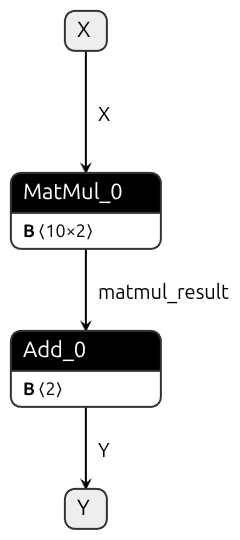
\includegraphics[height=5cm]{imgs/simple_net.onnx.png}
    \end{minipage}
    \caption{A simple \vnnlib{} specification which declares a network with a single input and output tensor. An example of one of the many possible ONNX models compatible with this declaration is shown on the right. Note that the variable names \texttt{X} and \texttt{Y} for the declared inputs and outputs do not have to match the node names in the ONNX file.}
    \label{fig:simple-query}
\end{figure}


It is important to clarify that a network declaration only declares an \emph{interface} and does not reference any particular ONNX network model. 
When passing a query and a network model to the verifier, the name of the network does not need to match the name of the ONNX model file. 
Instead, as described in Section~\ref{sec:verify_command}, the user will explicitly associate a network declaration to the relevant model file via the command line.
Neither do the declared names of the inputs and outputs need to match the names of the input and output nodes within the ONNX model file. This flexibility allows many different alternative ONNX models to be compatible with the same query.

All variable names follow the same syntax conventions: they are case-sensitive, must start with a letter, and may only contain letters, digits and underscores. All variable names must be unique within the query (see Section~\ref{sec:scoping_and_typing} for more detailed scoping rules). 


% The \texttt{@} character is a reserved character which is used to denote multiple applications of the same network, for the purpose of defining  hyperproperties such as monotonicity. For example \texttt{(declare-network acasXu@1 ...)} and \texttt{(declare-network acasXu@2 ...)} define two networks that are both instances of the same ONNX model,  denoted as \texttt{acasXu} in the command line interface of the verifier (See Chapter~\ref{sec:solver_interface} for more details).

\subsection{Assertions}

The list of assertions constrain the variables introduced by the network declarations. \vnnlib{} assertions are quantifier-free logical formulas and are defined using parenthesized \texttt{(assert\ldots)} expressions. 
They use an SMT-LIB-like reverse Polish notation syntax with the operator preceding its operands.
An assertion is a logical formula that may include logical connectives, relational comparisons, and arithmetic expressions over declared tensors and constants.
The final satisfiability problem is then the conjunction of all the assertions.
 
\paragraph{Constants}

Numeric constant values may be referenced using basic standard integer or floating point syntax (e.g. \inlinevnn{0}, \inlinevnn{0.0}, \inlinevnn{-0.5}). 

\paragraph{Variables} 

Standard indexing notation may be used to refer to a specific element within the tensor variable. For example, Line 6 in Figure~\ref{fig:simple-query} uses \inlinevnn{X[0,2]}, to refer to the value of the element of the input tensor at row~0, column~2. All indices are zero based and currently the number of indices provided must be equal to the number of dimensions of the variable, i.e. partial indexing is not allowed.

\paragraph{Arithmetic expressions}

One forms arithmetic expressions by recursively combining constant and variable values via prefix notation. Currently the following operators are supported:
\begin{itemize}
	\item \inlinevnn{(- a)}: Negation of a term.
    \item \inlinevnn{(+ a b ...)}: Addition of two or more terms. 
    \item \inlinevnn{(* a b ...)}: Multiplication of two or more terms. 
    \item \inlinevnn{(- a b ...)}: Subtraction of two or more terms. Note that subtraction associates to the left, e.g. \inlinevnn{(- 1 2 3 4)} is the same as \inlinevnn{(- (- (- 1 2) 3) 4)} .
\end{itemize}
Arithmetic operations currently only operate over individual tensor elements and cannot be used to operate over multi-dimensional tensors (see Section~\ref{sec:scoping_and_typing} for detailed typing rules).

\paragraph{Comparisons}

The comparison operators \inlinevnn{<=}, \inlinevnn{>=}, \inlinevnn{<}, \inlinevnn{>}, \inlinevnn{=}, \inlinevnn{!=} can be used to compare the values of two arithmetic operations.
For example, \inlinevnn{(<= a b)} returns true if $a$ is less than or equal to $b$.
    
\paragraph{Boolean expressions} 

One forms boolean expressions by recursively combining comparisons via the following supported logical connectives:
\begin{itemize}
    \item \inlinevnn{(and a b ...)}: Conjunction of two or more terms.
    \item \inlinevnn{(or a b ...)}: Disjunction of two or more terms.
\end{itemize}

\subsection{More complex network declarations}
\label{sec:complex-networks-decls}

Although queries often relate the input of a single network to its output in some way, \vnnlib{} supports more complex queries. The neural network may have multiple input or output nodes, or the query may refer to intermediate hidden layers of the network or it may relate the behaviour of multiple networks. The query language supports all of these use cases.

\subsubsection{Multiple input and output declarations}

Neural network that accept multi-modal input or produce multi-modal output are becoming increasingly common. 
For example, the network in Figure~\ref{fig:multi-inputs-outputs} shows a model that takes both an image and meta-data about that image as inputs, and outputs both a bounding box around an identified object of interest and a probability distribution over the possible class that the object belongs to. 

The query language supports such networks by allowing a network declaration to declare an arbitrary number of input and output declarations. The question is then how is the list of declared inputs and outputs mapped to the list of inputs and outputs nodes in the ONNX model. There are two ways to specify this mapping: 
\begin{itemize}
    \item \textbf{By order:} the default is that declared inputs and outputs are mapped to the ONNX graph's inputs and outputs by matching the order of declaration in the query to the order of declaration in the ONNX model file. This is demonstrated in the top code snippet in Figure~\ref{fig:multi-inputs-outputs}
    \item \textbf{By name:} alternatively, variables can be explicitly mapped using the names of the nodes within the ONNX graph. If this method is used, all input and output variables within that network declaration must be given an explicit ONNX node name. This is demonstrated in the bottom code snippet in Figure~\ref{fig:multi-inputs-outputs}.
\end{itemize}

\begin{figure}[h!]
    \centering
    \begin{lstlisting}[style=lbnf]
(declare-network multi_io_net
    (declare-input  image    float32 [1,3,224,224])
    (declare-input  metadata float32 [1,10])
    (declare-output bbox     int16   [1 4])
    (declare-output logits   float32 [1,1000])
)\end{lstlisting}

    \begin{lstlisting}[style=lbnf]
(declare-network multi_io_net
    (declare-input  metadata float32 [1,10]        "metadata")
    (declare-input  image    float32 [1,3,224,224] "image")
    (declare-output logits   float32 [1,1000]      "logits")
    (declare-output bbox     int16   [1,4,2]       "bbox")
)\end{lstlisting}

    \vspace{0.5cm}
    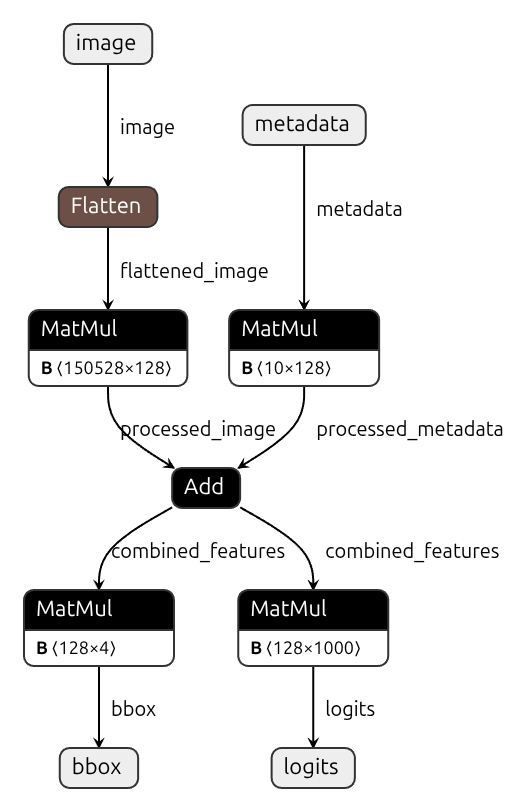
\includegraphics[width=\textwidth]{imgs/multi_io_net.onnx.png}
    \caption{A \vnnlib{} network declaration with multiple inputs/outputs. The first code snippet shows the declared inputs and outputs mapped to the ONNX inputs and outputs nodes by declaration order, while the second snippet shows them explicitly mapped by the name of the ONNX node.}
    \label{fig:multi-inputs-outputs}
\end{figure}


\subsubsection{Hidden output declarations}
\label{sec:hidden-output-declarations}

In some use cases it is desirable to constrain the result of intermediate computation at the output of hidden nodes within the network. For example, when reasoning about the encodings in an encoder-decoder architecture or when reasoning about attention mechanisms. This can be achieved by declaring hidden nodes using the \texttt{declare-hidden} keyword. This declaration includes a variable name for use within the \vnnlib{} specification,  its element type, its tensor shape, and crucially, a string identifier that specifies the corresponding node name in the ONNX graph.  Multiple hidden nodes can be trivially declared within a single network declaration. Figure~\ref{fig:hidden-node} shows a \vnnlib{} network declaration with a hidden node.

\begin{figure}[h!]
    \begin{minipage}[c]{0.76\textwidth}
        \begin{lstlisting}[style=lbnf]   
(declare-network encoder
    (declare-input  X float64 [1,28,28])
    (declare-hidden Z float64 [1,128] "hidden")
    (declare-output Y float64 [1,10])
)\end{lstlisting}
    \end{minipage}%
    \begin{minipage}[c]{0.21\textwidth}
        \centering
        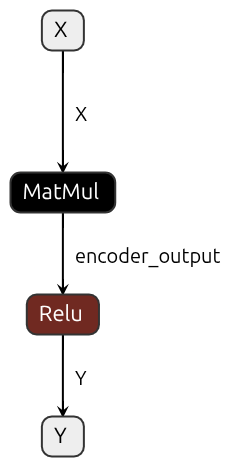
\includegraphics[height=6cm]{imgs/encoder_net.onnx.png}
    \end{minipage}
    \caption{A \vnnlib{} network declaration that declares a hidden node}
    \label{fig:hidden-node}
\end{figure}

The hidden node declaration crucially refers to the uniquely identified outputs of a node, rather than the node (or operator) itself. It declares that an output of the node is to be used as a variable in the \vnnlib{} query.

\subsubsection{Multiple networks}
\label{sec:multiple-network}

Often you may want to relate the behaviour of one neural network to that of another. Classic examples include: teacher-student networks where you try to train a smaller, more efficient network to mimic the output of the larger network, or observer-controller architectures.

\vnnlib{} supports defining multiple networks in by including multiple network declarations in the same query. Figure~\ref{fig:multiple-networks} 
shows an example which declares two networks representing a teacher and a student network.

\begin{figure}[h!]
    \begin{minipage}[c]{0.64\textwidth}
        \begin{lstlisting}[style=lbnf]
(declare-network teacher
    (declare-input  TX float32 [1,32])
    (declare-output TY float32 [1,2])
)

(declare-network student
    (declare-input  SX float16 [1,32])
    (declare-output SY float16 [1,2])
)\end{lstlisting}
    \end{minipage}
    \begin{minipage}[c]{0.35\textwidth}
        \centering
        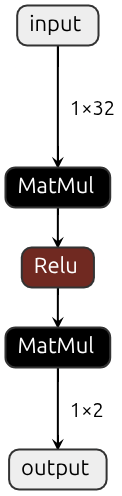
\includegraphics[height=7cm]{imgs/teacher_net.onnx.png}
        \vspace{0.5cm} 
        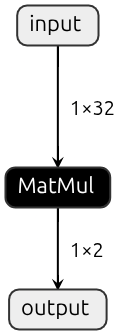
\includegraphics[height=5cm]{imgs/student_net.onnx.png}
    \end{minipage}
    \caption{A pair of \vnnlib{} network declarations that allows the referencing of multiple networks within a single query.}
    \label{fig:multiple-networks}
\end{figure}

For some use cases involving multiple networks (e.g. proving monotonicity), each \texttt{declare-network} declaration is intended to map to the same network implementation. In this case, the \texttt{equal-to} declaration may be used as shown in Figure~\ref{fig:multiple-equal-networks} to inform the verifier of this fact. An \texttt{equal-to} declaration must reference a network declaration which has identical \texttt{declare-input} and \texttt{declare-output} declarations (modulo the variable names). It \emph{is} possible to have a different list of \texttt{declare-hidden} declarations in the two networks. However if a \texttt{declare-hidden} declaration that references the same ONNX node is present in both networks then those \texttt{declare-hidden} declarations must be identical modulo the variable names. 
 Finally, marking a \texttt{declare-network} declaration as equal to one another means that it is not necessary to provide an implementation for that declaration when calling the verifier (see Section~\ref{sec:verify_command} for details).
 
\begin{figure}[h!]
    \begin{minipage}[c]{0.64\textwidth}
        \begin{lstlisting}[style=lbnf]
(declare-network f
    (declare-input  A float32 [1,10])
    (declare-output B float32 [1,2])
)

(declare-network f-copy
    (equal-to f)
    (declare-input  C float32 [1,10])
    (declare-output D float32 [1,2])
)\end{lstlisting}
    \end{minipage}
    \begin{minipage}[c]{0.35\textwidth}
        \centering
        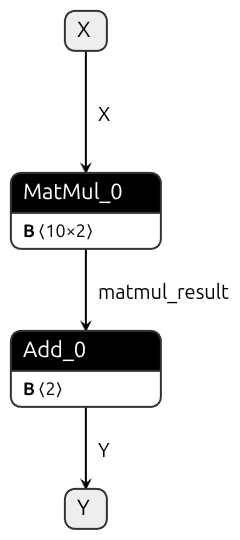
\includegraphics[height=5cm]{imgs/simple_net.onnx.png}
    \end{minipage}
    \caption{A pair of \vnnlib{} network declarations that reference the same ONNX network.}
    \label{fig:multiple-equal-networks}
\end{figure}

In other use cases involving multiple networks (e.g. proving local equivalence after retraining or after quantisation), each network declaration will be mapped to a network with the same graph structure but with different weights. In this case, the \texttt{isomorphic-to} declaration may be used as shown in Figure~\ref{fig:multiple-isomorphic-networks}. An \texttt{isomorphic-to} declaration must reference a network declaration which has identical list of \texttt{declare-input} and \texttt{declare-output} declarations, modulo the variable names and the element type. As with the \texttt{equal-to} declaration, it \emph{is} possible to have a different list of \texttt{declare-hidden} declarations in the two \texttt{declare-network} declarations. However if a \texttt{declare-hidden} declaration that references the same ONNX node is present in both then those \texttt{declare-hidden} declarations must be identical modulo the variable names and element types.

\begin{figure}[h!]
    \begin{minipage}[c]{0.64\textwidth}
        \begin{lstlisting}[style=lbnf]
(declare-network f
    (declare-input  A float32 [1,10])
    (declare-output B float32 [1,2])
)

(declare-network g
    (isomorphic-to f)
    (declare-input  C float32 [1,10])
    (declare-output D float32 [1,2])
)\end{lstlisting}
    \end{minipage}
    \begin{minipage}[c]{0.35\textwidth}
        \centering
        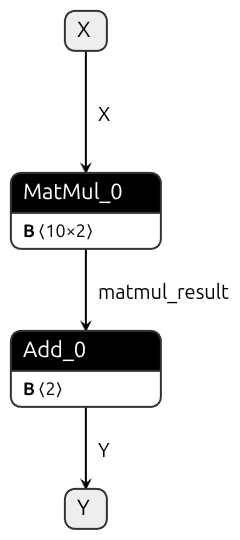
\includegraphics[height=5cm]{imgs/simple_net.onnx.png}
        \vspace{0.5cm} 
        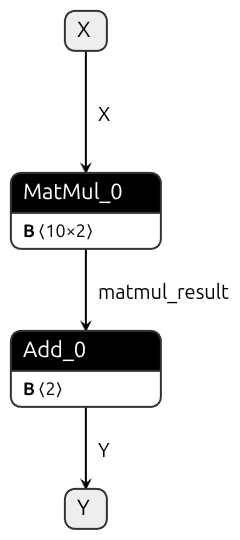
\includegraphics[height=5cm]{imgs/simple_net.onnx.png}
    \end{minipage}
    \caption{A pair of \vnnlib{} network declarations that reference isomorphic ONNX networks.}
    \label{fig:multiple-isomorphic-networks}
\end{figure}

There are two additional restrictions to their use:
\begin{enumerate}
\item A \texttt{declare-network} declaration must contain at most one \texttt{equal-to} or \texttt{isomorphic-to} declaration.
\item An \texttt{equal-to} or \texttt{isomorphic-to} declaration cannot reference another network declaration that also contains an \texttt{equal-to} or \texttt{isomorphic-to}. 
\end{enumerate}
Due to the transitivity of equality and isomorphism, these restrictions do not reduce the expressive power of this feature, and make the dependencies easier to track by the verifiers.

While a verifier may make use of the \texttt{equal-to} and \texttt{isomorphic-to} declarations internally to optimise its representation and reasoning about the provided networks, it is not required to.



\subsection{Comments and whitespace}

Comments in \vnnlib{} are denoted by a semicolon (\texttt{;}) and extend to the end of the line. They are used for annotation, explaining logic, or providing additional context. Whitespace in \vnnlib{} is used to separate tokens and improve readability and can include spaces, tabs, and newlines. Additional whitespace beyond the minimal necessary to separate tokens is ignored.


\section{Typing}
\label{sec:scoping_and_typing}
The scoping and typing judgments for the language are given in \autoref{fig:scoping-network-decls}, \autoref{fig:typing-arithExpr} and \autoref{fig:typing-boolExpr-query}. 
Network declarations are used to construct the static context ($\Gamma$) which is then used to type the globally-scoped variables and literals used in the assertions of a query.

A \vnnlib{} query is well-scoped if it satisfies the following criteria:
\begin{enumerate}
    \item All variables are declared before they are referenced.
    \item All variable names are unique.
    \item An equivalence statement in a network declaration must point to another network declaration that does not have a congruence statement.
\end{enumerate}
A \vnnlib{} query is said to be \textit{well-typed}, if it satisfies the following criteria.
\begin{itemize}
    \item All variables have a valid ONNX element type.
    \item Variables are \textit{strictly-typed}; so all variable references must match the expected element type in the context where it is substituted.
\end{itemize}

Although some ONNX types can be soundly cast for operations in certain cases, for example, a \textit{float16} can be added safely to a \textit{float32} if the expected type of evaluated expression is a \textit{float32}, the \vnnlib{} standard does not permit such implicit casting.
If a query is agnostic to the element type of variables, it should be declared with the \textit{Real} type.

\begin{figure}
    \begin{minipage}[t]{\linewidth}
    \resizebox{0.9\linewidth}{!}{
        \begin{mathpar}
            \inferrule*[Right=Input Declaration]{
            }{
                \Gamma \vdash (\texttt{declare-input}~v~\tau~s) : \Gamma[v \rightarrow (\tau,s,\texttt{input})]
            }
            \\
            \inferrule*[Right=Hidden Declaration]{
            }{
                \Gamma \vdash (\texttt{declare-hidden}~v~\tau~s) : \Gamma[ v \rightarrow (\tau,s,\texttt{hidden})]
            }
            \\
            \inferrule*[Right=Output Declaration]{
            }{
                \Gamma \vdash (\texttt{declare-output}~v~\tau~s) : \Gamma[ v \rightarrow (\tau,s,\texttt{output})]
            }
            \\ \\
            \hspace*{5em}
            \inferrule*[]{
                    {\begin{array}{lll}
                    \Gamma_0 &\vdash I_1 &: \Gamma_1 
                    \\
                    &\vdots
                    \\
                    \Gamma_{n-1} &\vdash I_n &: \Gamma_n 
                    \end{array}}
                    \\
                    {\begin{array}{lll}
                    \Gamma_n &\vdash H_1 &: \Gamma_{n+1} 
					\\                    
                    &\vdots 
					\\                    
                    \Gamma_{m+n-1} &\vdash H_m &: \Gamma_{m+n} 
                    \end{array}}
					\\                  
                    {\begin{array}{lll}
                    \Gamma_{m+n} &\vdash O_1 &: \Gamma_{m+n+1} 
                    \\
					&\vdots
					\\
                    \Gamma_{m+n+o-1} &\vdash O_o &: \Gamma_{n+m+o} 
                    \end{array}}
            }{
                (\Gamma_0 , N_0) \vdash (\texttt{declare-network}~(I_1~...~I_n)~(H_1~...~H_m)~(O_1~...~O_o)) : (\Gamma_{n+m+o}, N_1)
            }
            \\
            \scalebox{0.9}{\textsf{\textsc{NetworkDeclaration}}}
            \end{mathpar}
        }
    \caption{Scoping judgments for network declarations}
    \label{fig:scoping-network-decls}
    \end{minipage}
\end{figure}

\begin{figure}
    \begin{minipage}[t]{1\textwidth}
        \resizebox{\textwidth}{!}{
        \begin{mathpar}
            \inferrule*[Right=Real Literal]{
                d \in \mathbb{R}
            }{
                \Gamma \vdash d : \text{Real}
            }
            \\
            \inferrule*[Right=Float64 Literal]{
                d \in \text{Float64}
            }{
                \Gamma \vdash d : \text{float32}
            }
            \\
            \vdots
            \\
            \inferrule*[Right=<ElementType> Literal]{
                d~\in~$T$ \quad \text{where}~$T$~\leftrightarrow\tau
            }{
                \Gamma \vdash d : \tau
            }
            \\
            \inferrule*[Right=Variable]{
                \Gamma [v] = (\tau,s,\mu) \quad \text{validIndices}~(i, s)
            }{
                \Gamma \vdash v~i : \tau
            }
            \\
            \inferrule*[Right=Negation]{
                \Gamma \vdash a : \tau
            }{
                \Gamma \vdash (\texttt{-}~a) : \tau
            }
            \\
            \inferrule*[Right=N-ary Operations]{
                \Gamma \vdash a_1 : \tau \quad ... \quad \Gamma \vdash a_n : \tau \quad \circledast \in \{\texttt{+}, \texttt{-}, \texttt{×}\}
            }{
                \Gamma \vdash (\circledast~a_1~...~a_n) : \tau
            }
        \end{mathpar}
        }
    \caption{Typing judgments of arithmetic expressions}
    \label{fig:typing-arithExpr}
    \end{minipage}
\end{figure}

\begin{figure}
    \begin{minipage}[t]{1\textwidth}
        \resizebox{\textwidth}{!}{
        \begin{mathpar}
            \inferrule*[Right=BoolExpr Comparisons]{
                \Gamma \vdash a_1 : \tau \quad \Gamma \vdash a_2 : \tau \quad \lozenge \in \{\texttt{>=}, \texttt{>}, \texttt{<}, \texttt{<=}, \texttt{==}, \texttt{!=}\}
            }{
                \Gamma \vdash (\lozenge~a_1~a_2) 
            }
            \\
            \hspace{1cm}
            \inferrule*[Right=BoolExpr Connectives]{
                \Gamma \vdash b_1 \quad ... \quad \Gamma \vdash b_n \quad \Box \in \{\texttt{and}, \texttt{or}\}
            }{
                \Gamma \vdash (\Box~b_1~...~b_n)
            }
            \\
            \inferrule*[Right=Assertion]{
                \Gamma \vdash b
            }{
                \Gamma \vdash (\texttt{assert}~b)
            }
            \\ \\
            \inferrule*[Right=Query]{
                \ensuremath{
                    \begin{array}{ccc}
                    \{\}~\vdash D_1 : \Gamma_1 & \Gamma_n \vdash A_1 \\
                    \Gamma_1~\vdash D_2 : \Gamma_2 & \Gamma_n \vdash A_2 \\
                    \vdots & \vdots \\
                    \Gamma_{n-1} \vdash D_n : \Gamma_n & \Gamma_n \vdash A_m
                    \end{array}
                }
            }{
                (V~(D_1~...~D_n)~(A_1,...,A_m))
            }
        \end{mathpar}
        }
    \caption{Typing judgments of boolean expressions and a \vnnlib{} query}
    \label{fig:typing-boolExpr-query}
    \end{minipage}
\end{figure}

\section{Semantics}
\label{sec:semantics}

The semantics of a \vnnlib{} query is defined in terms of the satisfiability problem it represents. A query is said to be \textit{satisfiable} if there exists an assignment of values to all/any of the the input tensors such that when the corresponding ONNX model(s) are evaluated, the set of assertions hold true. Conversely, a query is said to be \textit{unsatisfiable} if no such assignment exists.

Given that the actual semantics of a \vnnlib{} query is dependent on the semantics of the neural network representation i.e. on the underlying ONNX model(s) it is associated with, we can describe the semantics of a query as a higher order function from functions representing the declared ONNX networks to a satisfiability problem over the input assignments. 

The semantics are only well-defined if the query is well-scoped and well-typed, as described in Section~\ref{sec:scoping_and_typing}. Similarly, the semantics for the Declarations and Assertions can be described separately.

\myremark{
    The \vnnlib{} standard version 2.0 does not formalise the semantics of network congruence, or of hidden nodes.
}


\paragraph{Query}
\mytodo{Add description of equation}
\begin{multline}
\sem{V~(D_1,...,D_n)~(A_1,...,A_m)} = \\
    (\Delta_N : \prod^{n}_{i=1}~\sem{D_i}_N) \rightarrow~\exists~(\Delta_A : \prod^{n}_{i=1}~\sem{D_i}_A).\bigwedge^{m}_{i=1}~\semenv{A_i} \\
\end{multline}

\paragraph{Network Declarations}
The semantic context for a \vnnlib{} query is constructed from the Declarations of a \vnnlib{} query is a pair, which represents networks as a function from a product of input tensors to a product of output tensors (\autoref{eq:networkImplementations}), and the input assignments as the product of input tensors (\autoref{eq:inputAssignments}).

\begin{align}
    \sem{\texttt{declare-input}~v~\tau~s} &= \tau^s \label{eq:declInput}\\
    \sem{\texttt{declare-output}~v~\tau~s} &= \tau^s \label{eq:declOutput}\\
    \sem{\texttt{declare-network}~v~(I_1,...,I_n)~(O_1,...,O_m)}_N &= \prod^{n}_{i=1}~\sem{I_i} \rightarrow \prod^{m}_{i=1}~\sem{O_i} \label{eq:networkImplementations} \\
    \sem{\texttt{declare-network}~v~(I_1,...,I_n)~(O_1,...,O_m)}_A &= \prod^{n}_{i=1}~\sem{I_i} \label{eq:inputAssignments}
\end{align}

\paragraph{Assertions}
The semantics of an assertion uses a typing context $\Gamma$, that is constructed iteratively for the network declarations (\autoref{fig:scoping-network-decls}).
The semantics of arithmetic expressions (\autoref{eq:double} to \autoref{eq:minus}), and boolean comparative expressions (\autoref{eq:greaterEqual} to \autoref{eq:notEqual}) use typed ($\tau$) operators. The mapping of the equivalent ONNX operators \cite{onnxOperators} are given in \autoref{tab:onnx-operators}.\

\begin{equation*}
\begin{array}{llll}
    \semenv{\Gamma\vdash{d}:\tau} 
    &= d 
    \\
    \semenv{\Gamma\vdash{v~i}:\tau} 
    &= \begin{cases}
        \Delta_{A_i}^k & \text{if}~\Gamma[v]~= (\tau,s,\texttt{input})\\
        \Delta_{N}^k(\Delta_{A_i}^k) & \text{if}~\Gamma[v]~= (\tau,s,\texttt{output})\\
    \end{cases} 
    \\
    &\text{where}~k = \text{indexOf}~(g)\notag
    \\
    \semenv{\Gamma\vdash(\text{\texttt{-}}~a_1):\tau}
    &= -_\tau~\semenv{\Gamma\vdash{a_1}~:~\tau} 
    \\
    \semenv{\Gamma\vdash(\text{\texttt{+}}~a_1~...~a_n):\tau} 
    &= \sum^{\tau, n}_{i=1}\semenv{\Gamma\vdash{a_i}:\tau} 
    \\
    \semenv{\Gamma\vdash(\text{\texttt{*}}~a_1~...~a_n):\tau} 
    &= \prod^{\tau, n}_{i=1}\semenv{\Gamma\vdash{a_i}:\tau} 
    \\
    \semenv{\Gamma\vdash(\text{\texttt{-}}~a_1~...~a_n):\tau} 
    &= \semenv{\Gamma\vdash{a_1}:\tau}~+_\tau~(-_\tau~\tau.\sum^{n}_{i=2}\semenv{\Gamma\vdash{a_i}:\tau}) 
    \\
    \semenv{\Gamma\vdash(\text{\texttt{>=}}~a_1~a_2)} 
    &= \semenv{\Gamma\vdash{a_1}}~\geq_\tau~\semenv{\Gamma\vdash{a_2}}
    \\
    \semenv{\Gamma\vdash(\text{\texttt{> }}~a_1~a_2)} 
    &= \semenv{\Gamma\vdash{a_1}}~>_\tau~\semenv{\Gamma\vdash{a_2}} 
    \\
    \semenv{\Gamma\vdash(\text{\texttt{<=}}~a_1~a_2)} 
    &= \semenv{\Gamma\vdash{a_1}}~\leq_\tau~\semenv{\Gamma\vdash{a_2}} 
    \\
    \semenv{\Gamma\vdash(\text{\texttt{< }}~a_1~a_2)} 
    &= \semenv{\Gamma\vdash{a_1}}~<_\tau~\semenv{\Gamma\vdash{a_2}} 
    \\
    \semenv{\Gamma\vdash(\text{\texttt{==}}~a_1~a_2)} 
    &= \semenv{\Gamma\vdash{a_1}}~=_\tau~\semenv{\Gamma\vdash{a_2}} 
    \\
    \semenv{\Gamma\vdash(\text{\texttt{!=}}~a_1~a_2)} 
    &= \semenv{\Gamma\vdash{a_1}}~\neq_\tau~\semenv{\Gamma\vdash{a_2}}
    \\
    \semenv{\text{\texttt{and}}~b_1~...~b_n} &=\bigwedge^{n}_{i=1}\semenv{b_i}\\
    \semenv{\text{\texttt{or}}~b_1~...~b_n} &=\bigvee^{n}_{i=1}\semenv{b_i}\\
    \semenv{\text{\texttt{assert}}~b} &= \semenv{b}
\end{array}
\end{equation*}